% latex $fileNameWithoutExt; dvisvgm $fileNameWithoutExt --bbox=papersize --font-form=ttf --precision=3 --optimize=collapse-groups,group-attributes,simplify-text,simplify-transform
\documentclass[tikz, border=2mm]{standalone}
\usepackage{pgfplots}
\pgfplotsset{compat=1.18}
\begin{document}
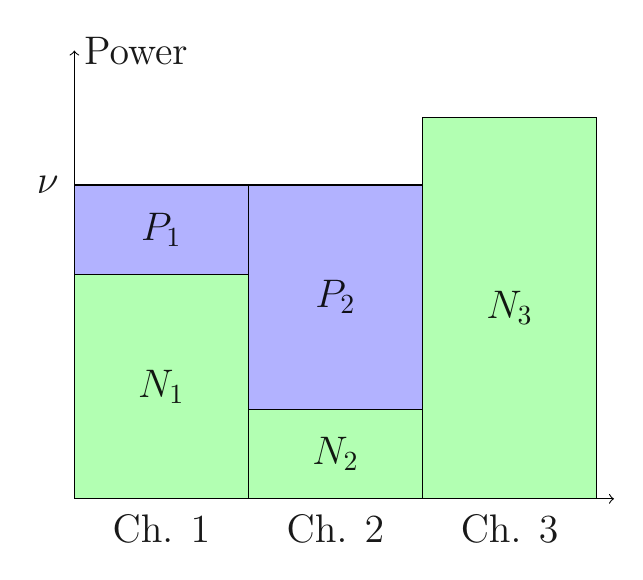
\begin{tikzpicture}
  \begin{axis}[
    ybar stacked,
    axis lines=center,
    clip=false,
    axis x line=bottom,
    axis y line=left,
    xmin=0.5,
    xmax=3.6,
    x tick style={draw=none},
    xtick={1,2,3},
    xticklabels={Ch. 1,Ch. 2, Ch. 3},
    ytick style={draw=none},
    ytick={70},
    yticklabels={$\nu$},
    ymin=0,
    ymax=100,
    ylabel={Power},
    y label style={anchor=west, align=left},
    text opacity=.9,
    font=\Large,
    axis line style=->,
    every axis plot/.append style={
      ybar,
      bar width=1,
      fill opacity=.3,
      draw,
    }
  ]
    \addplot[fill=green, nodes near coords=$N_{\pgfmathtruncatemacro\x{\coordindex+1}\x}$]coordinates{(1,50)(2,20)(3,85)};
    \addplot[fill=blue, nodes near coords=$P_{\pgfmathtruncatemacro\x{\coordindex+1}\x}$]coordinates{(1,20)(2,50)};
  \end{axis}
\end{tikzpicture}
\end{document}
